\documentclass{article}


\usepackage[utf8]{inputenc}
\usepackage[english]{babel}
\usepackage{fancyhdr}
\usepackage{lastpage}
\usepackage{hyperref}
\usepackage{titling}
\usepackage{titlesec}
\usepackage{graphicx}
\usepackage{wrapfig}
\usepackage{listings}
\usepackage{textcomp}
\usepackage{scrextend}
%\graphicspath{ {/} }

\pagestyle{fancy}
\fancyhf{}

\lstset{basicstyle=\ttfamily,
escapeinside={||},
mathescape=true}

% last page seems to need two runs, which I assume actually means you need to create the bulid and render files in a
% certain order
% https://tex.stackexchange.com/questions/28708/why-does-pagereflastpage-give-me-rather-than-page-number-of-the-last-pag
\rfoot{\thepage \hspace{1pt} of \pageref{LastPage}}

% define subtitle command
\newcommand{\subtitle}[1]{%
	\posttitle{%
		\par\end{center}
		\begin{center}\large#1\end{center}
		\vskip0.5em}%
}

% define paragraph to be a subsubsubsection
\titleclass{\subsubsubsection}{straight}[\subsection]

\newcounter{subsubsubsection}[subsubsection]
\renewcommand\thesubsubsubsection{\thesubsubsection.\arabic{subsubsubsection}}
\renewcommand\theparagraph{\thesubsubsubsection.\arabic{paragraph}} % optional; useful if paragraphs are to be numbered

\titleformat{\subsubsubsection}
  {\normalfont\normalsize\bfseries}{\thesubsubsubsection}{1em}{}
\titlespacing*{\subsubsubsection}
{0pt}{3.25ex plus 1ex minus .2ex}{1.5ex plus .2ex}

\makeatletter
\renewcommand\paragraph{\@startsection{paragraph}{5}{\z@}%
  {3.25ex \@plus1ex \@minus.2ex}%
  {-1em}%
  {\normalfont\normalsize\bfseries}}
\renewcommand\subparagraph{\@startsection{subparagraph}{6}{\parindent}%
  {3.25ex \@plus1ex \@minus .2ex}%
  {-1em}%
  {\normalfont\normalsize\bfseries}}
\def\toclevel@subsubsubsection{4}
\def\toclevel@paragraph{5}
\def\toclevel@paragraph{6}
\def\l@subsubsubsection{\@dottedtocline{4}{7em}{4em}}
\def\l@paragraph{\@dottedtocline{5}{10em}{5em}}
\def\l@subparagraph{\@dottedtocline{6}{14em}{6em}}
\makeatother

\setcounter{secnumdepth}{4}
\setcounter{tocdepth}{4}


\title{Steem}
\subtitle{An incentivized, blockchain-based social media platform.}
\date{March 2016}
\author{
	Daniel Larimer\
	\and
	Ned Scott\
	\and
	Valentine Zavgorodnev\
	\and
	Benjamin Johnson\
	\and
	James Calfee\
	\and
	Michael Vandeberg
	}

\pagenumbering{arabic}

\begin{document}

	\renewcommand \thesection{\roman{section}}

	\maketitle

	\newpage

	\section{Abstract}

		Steem is a blockchain database that supports community building and social interaction with cryptocurrency rewards. Steem combines concepts from social media with lessons learned from building cryptocurrencies and their communities. An important key to inspiring participation in any community, currency or free market economy is a fair accounting system that consistently reflects each person's contribution. Steem is the first cryptocurrency that attempts to accurately and transparently reward an unbounded number of individuals who make \textit{subjective contributions} to its community.

	\newpage

	\section{Table of Contents}

	\tableofcontents

	\newpage

	\setcounter{section}{0}

	\renewcommand \thesection{\arabic{section}}

	\section{Introduction}

	    \paragraph{}
			Collectively, user-generated content has created billions of dollars worth of value for the shareholders of social media companies, such as Reddit, Facebook, and Twitter. \textbf{In 2014, Reddit hypothesized that its platform would be improved if everyone who contributed to reddit.com by posting stories, adding comments or voting were rewarded with a fair share in Reddit, Inc\footnote{Reddit's Cryptocurrency, Forbes, Erika Morphy, October 2014,\newline\url{http://www.forbes.com/sites/erikamorphy/2014/10/01/reddits-cryptocurrency-could-have-many-uses/\#4e07b05332b9}}}. Steem aims to support social media and online communities by returning much of its value to the people who provide valuable contributions by rewarding them with cryptocurrency, and through this process create a currency that is able to reach a broad market, including people who have yet to participate in any cryptocurrency economy.

		\paragraph{}
			There are some key principles that have been used to guide the design of Steem. The most important principle is that everyone who contributes to a venture should receive pro-rata ownership, payment or debt from the venture. This principle is the same principle that is applied to all startups as they allocate shares at founding and during subsequent funding rounds.

		\paragraph{}
			The second principle is that all forms of capital are equally valuable. This means that those who contribute their scarce time and attention toward producing and curating content for others are just as valuable as those who contribute their scarce cash. This is the sweat equity principle\footnote{Sweat Equity, Investopedia,\newline\url{http://www.investopedia.com/terms/s/sweatequity.asp}} and is a concept that prior cryptocurrencies have often had trouble providing to more than a few dozen individuals.

		\paragraph{}
			The third principle is that the community produces products to serve its members. This principle is exempli ed by credit unions, food co-ops, and health sharing plans, which serve the members of their community rather than sell products or services to people outside the community.

		\paragraph{}
			The Steem community provides the following services to its members:

		\begin{enumerate}
			\item A source of curated news and commentary.
			\item A means to get high quality answers to personalized questions.
			\item A stable cryptocurrency pegged to the U.S. dollar.
			\item Free payments.
			\item Jobs providing above services to other members.
		\end{enumerate}

		\paragraph{}
			Steem's purposeful realignment of economic incentives has the potential to produce fairer and more inclusive results for everyone involved than the social media and cryptocurrency platforms that have gone before it. This paper will explore the existing economic incentives and demonstrate how Steem's incentives may result in better outcomes for most participants.

		\subsection{Recognizing Contribution}

			\paragraph{}
				Steem is designed from the ground up to address the major barriers to adoption and monetization of a social media based economy. Our thesis is that the same techniques used to grow major social media platforms can be used to bootstrap a successful cryptocurrency. Economic incentives enabled by cryptocurrency can dramatically facilitate the growth of a new social media platform. It is the synergy between cryptocurrency and social media that we believe may give Steem a powerful advantage in the market.

			\paragraph{}
				The challenge faced by Steem is deriving an algorithm for scoring individual contributions that most community members consider to be a fair assessment of the subjective value of each contribution. In a perfect world, community members would cooperate to rate each other's contribution and derive a fair compensation. In the real world, algorithms must be designed in such a manner that they are resistant to intentional manipulation for profit. Any widespread abuse of the scoring system could cause community members to lose faith in the perceived fairness of the economic system.

			\paragraph{}
				Existing platforms operate on a one-user, one-vote principle. This creates an environment where rankings can be manipulated by sybil attacks and the service providers must pro-actively identify and block abusers. People already attempt to manipulate the Reddit, Facebook, and Twitter scoring algorithms when the only reward is web traffic or censorship.

			\paragraph{}
				The fundamental unit of account on the Steem platform is STEEM, a crypto currency token. Steem operates on the basis of one-STEEM, one-vote. Under this model, individuals who have contributed the most to the platform, as measured by their account balance, have the most influence over how contributions are scored. Furthermore, Steem only allows members to vote with STEEM when it is committed to a multi-year vesting schedule. Under this model, members have a financial incentive to vote in a way that maximises the long term value of their STEEM.

			\paragraph{}
				Steem is designed around a relatively simple concept: \textit{everyone's meaningful contribution to the community should be recognized for the value it adds.} When people are recognized for their meaningful contributions, they continue contributing and the community grows. Any imbalance in the give and take within a community is unsustainable. Eventually the givers grow tired of supporting the takers and disengage from the community.

			\paragraph{}
				The challenge is creating a system capable of identifying what contributions are needed and their relative worth in a way that can scale to an unbounded number of people.

			\paragraph{}
				A proven system for evaluating and rewarding contributions is the free market. The free market can be viewed as a single community where everyone trades with one another and rewards are allocated by profit and loss. The market system rewards those who provide value to others and punishes those who consume more value than they produce. The free market supports many different currencies and money is simply a commodity that everyone finds easy to exchange.

			\paragraph{}
				Since the free market is a proven system, it is tempting to try to create a free-market system where content consumers directly pay content producers. However, direct payment is inefficient and not really viable for content creation and curation. The value of most content is so low relative to the cognitive, financial, and opportunity costs associated with making a payment that few readers choose to tip. The abundance of free alternatives means that enforcing a 'paywall' will drive readers elsewhere. There have been several attempts to implement per-article micropayments from readers to authors, but none have become widespread.

			\paragraph{}
				Steem is designed to enable effective micropayments for all kinds of contribution by changing the economic equation. Readers no longer have to decide whether or not they want to pay someone from their own pocket, instead they can vote content up or down and Steem will use their votes to determine individual rewards. This means that people are given a familiar and widely used interface and no longer face the cognitive,  nancial, and opportunity costs associated traditional micropayment and tipping platforms.

			\paragraph{}
				Voting input from community members is critical for Steem to accurately allocate payments to contributors. Voting can therefore be viewed as a crucial contribution and worthy of rewards on its own. Some platforms, such as Slashdot, use meta-moderation\footnote{\textbf{Meta-moderation} is a second level of comment moderation. Users are invited to rate a moderator's decision in order to improve moderation.\newline\url{https://en.wikipedia.org/wiki/Meta-moderation_system}} as a way to rank and reward honest moderators. Steem chooses to reward those who contribute the most to the total promotion of a piece of content and rewards the voters proportional to the ultimate reward paid to the content creator.

			\paragraph{}
				There are other forms of contribution that Steem recognizes and rewards using objective metrics. Among these are: transaction validation, proof of work mining, liquidity rewards, and reporting of misbehaving block producers.

	\section{Ways to Contribute}

		This section outlines the ideas behind Steem and its rewards for people who provide meaningful and measurable contributions to the Steem community.

		\subsection{Capital Contributions}

			\paragraph{}
				There are two items a community can offer to attract capital: debt and ownership. Those who buy ownership profit when the community grows but lose if the community shrinks. Those who buy debt are guaranteed a certain amount of interest but do not get to participate in any profits realized by the growth of the community. Both types of capital contributions are valuable to the growth of the community and value of its currency. Additionally there are two ways ownership can be held: liquid and vesting. Vesting ownership makes a long-term commitment and cannot be sold for a minimum period of time.

			\paragraph{}
				The Steem network calls these different asset classes Steem (STEEM), Steem Power (SP), and Steem Dollars (SMD).

		\subsection{Steem (STEEM)}

			\paragraph{}
				Steem is the fundamental unit of account on the Steem blockchain. All other tokens derive their value from the value of STEEM. Generally speaking STEEM should be held for short periods of time when liquidity is needed. Someone looking to enter or exit the Steem platform will have to buy or sell STEEM. Once STEEM has been purchased it should be converted into SP or SMD to mitigate the impact of dilution over the long-term.

			\paragraph{}
				STEEM is constantly increasing in supply by 100\% per year due to non-SMD incentives. Someone who holds STEEM without converting it to SP is diluted by approximately 0.19\% per day. While the rate may appear high, for transactions that take less than 10 days, it is still cheaper than credit card processing fees. Furthermore, the daily token creation is insigni cant next to the daily volatility.

			\paragraph{}
				Someone who buys Bitcoin or any other cryptocurrency and sells it 10 days later could easily lose 3\% or more due to price fluctuations. Someone who buys Bitcoin and then sells it the same day will usually pay more than 0.4\% in market fees alone. In other words, the in ation rate is effectively insignificant during the period of time the typical individual will hold STEEM.

			\paragraph{}
				The majority of inflation is actually an accounting artifact rather than true reallocation of wealth. 90\% of non-SMD in ation is distributed back to existing holders of STEEM proportional to the STEEM value of their SP balance, making in ation more of a "split". Only about 10\% of non-SMD in ation redistributes ownership in the network.

		\subsection{Steem Power (SP)}

			\paragraph{}
				Start up companies require long-term capital commitment. Those who invest their money in a startup expect to wait years before they can sell their shares and realize their profits. Without long-term commitment, a startup seeking to raise additional capital through the sale of additional shares would be competing with existing shareholders looking to exit. Savvy investors want their capital contributions to grow the company, but growth cannot happen if the new capital is given away to those looking to exit.

			\paragraph{}
				There is significant value to having long-term commitment because it enables communities to make long-term plans. Long term commitment of stakeholders also causes them to vote for long-term growth rather than short-term pumps.

			\paragraph{}
				In the cryptocurrency space, speculators jump from cryptocurrency to cryptocurrency based mostly on which one is expected to have short-term growth. Steem wants to build a community that is mostly owned and entirely controlled by those with a long-term perspective.

			\paragraph{}
				Because Steem wants to encourage long-term growth, it is hardwired to allocate 9 STEEM to Steem Power (SP) stakeholders for every 1 STEEM it creates to fund growth through contribution incentives. Over time this drives the ratio of the total STEEM value of Steem Power balances to the total of STEEM balances toward 9:1 . (It seems likely that the ratio will be somewhat greater than 9:1 due to continued net Powering Up of the newly printed STEEM.) It also means that long-term holders are almost completely protected from the dilution used to fund growth.

			\paragraph{}
				SP can only be converted back to STEEM over 2 years via 104 equal weekly payments. '1 SP' can be viewed as a share in a pool of STEEM. The network automatically adds STEEM to the pool every block. At any time users can convert their STEEM into SP at the same ratio as STEEM in the vesting pool to total SP. Converting STEEM to SP does not dilute existing holders of SP. Likewise, every time SP is converted back to STEEM it is done at the current ratio. Individuals are guaranteed to have more STEEM in the future than they have when they  rst convert from STEEM to SP.

			\paragraph{}
				SP balances are non-transferrable and non-divisible except via the automatically recurring conversion requests. This means that SP cannot be easily traded on cryptocurrency exchanges.

			\paragraph{}
				SP is a requirement for voting for or against content. This means that SP is an access token that grants its holders exclusive powers within the Steem platform.

			\paragraph{}
				 Transferring from STEEM to SP is referred to as powering up while transferring from SP to Steem is referred to as "powering down." For example, one can power down their STEEM over a period of two years, yet one can power up their STEEM instantly.

		\subsection{Steem Dollars (SMD)}

			\paragraph{}
				Stability is an important feature of successful global economies. Without stability, individuals across the world could not have low cognitive costs while engaging in commerce and savings. Because stability is an important feature of successful economies, Steem Dollars were designed as an attempt to bring stability to the world of cryptocurrency and to the individuals who use the Steem network.

			\paragraph{}
				Steem Dollars are created by a mechanism similar to convertible notes, which are often used to fund startups. In the startup world, convertible notes are short-term debt instruments that can be converted to ownership at a rate determined in the future, typically during a future funding round. A blockchain based token can be viewed as ownership in the community whereas a convertible note can be viewed as a debt denominated in any other commodity or currency. The terms of the convertible note allow the holder to convert to the backing token with a minimum notice at the fair market price of the token. Creating token-convertible-dollars enables blockchains to grow their network effect while maximizing the return for token holders.

			\paragraph{}
				Steem Dollars are referred to with the symbol SMD, an acronym for Steem Dollars. Creating SMD requires a combination of a reliable price feed, rules to prevent abuse, and liquidity. Providing a reliable price feed involves three factors: minimizing the impact of an incorrect feed, maximizing the cost of producing an incorrect feed, and minimizing the importance of timing.

			\subsubsection{Minimizing Fraudulent Feeds}

				\paragraph{}
					SP holders elect individuals to publish price feeds. These elected individuals are presumably trusted by those who have a vested interest in the quality of the feed. By paying those who are elected, Steem creates market competition to earn the right to produce feeds. The more the feed producers are paid the more they have to lose by publishing false information.

				\paragraph{}
					Given a set of trusted and elected feed producers, the actual price used for conversions can be derived as the median of the feeds. In this way if any minority of individual feed producers produce outliers they have minimal impact on the actual median while still having the ability impact their reputation.

				\paragraph{}
					Even if all feed producers are honest, it is possible for the majority of feed producers to be impacted by events beyond their control. The Steem network is designed to tolerate short-term corruption of the median price feed while the community actively works to correct the issue. One example of an issue that may take some time to correct is short-term market manipulation. Market manipulation is difficult and expensive to maintain for long periods of time. Another example would be the failure of a centralized exchange or the corruption of the data published by the exchange.

				\paragraph{}
					Steem factors out short-term price fluctuations by using the median price over a period of one week. The median published feed is sampled every hour on the hour.

				\paragraph{}
					As long as the price feed corruption lasts for less than half the moving median time window it will have minimal impact on the conversion price. In the event the feed does get corrupted, network participants will have an opportunity to vote-out corrupt feed producers before the corrupted feed can impact the actual conversion price. Perhaps more importantly, it gives feed producers an opportunity to detect and correct issues before their feeds start impacting the price.

				\paragraph{}
					With a one week window, community members have three and a half days to respond to any issues that come up.

			\subsubsection{Mitigating Timing Attacks}

				\paragraph{}
					Market participants have access to information faster than the blockchain's one week moving median conversion price can react. This information could be used to benefit of traders at the expense of the community. If there is a sudden increase in the value of STEEM traders could request conversion of their SMD at the old, lower price, and then sell the STEEM they receive a the new higher price with minimal risk.

				\paragraph{}
					Steem levels the playing field by requiring all conversion requests to be delayed for one week. This means that neither the traders nor the blockchain has any information advantage regarding the price at the time the conversion is executed.

			\subsubsection{Minimizing Abuse of Conversions}

				\paragraph{}
					If people could freely convert in both directions then traders could take advantage of the blockchains conversion rates by trading large volumes without changing the price. Traders who see a massive run up in price would convert to SMD at the high price (when it is most risky) and then convert back after the correction. The Steem protocol protects the community from this kind of abuse by only allowing people to convert from SMD to STEEM and not the other way around.

				\paragraph{}
					The blockchain decides how and when to create SMD and who should get it. This keeps the rate of SMD creation stable and removes most avenues of abuse.

			\subsubsection{Liquidity}

				\paragraph{}
					Just because SMD can be converted to a dollars worth of STEEM at a fair price in a reasonable amount of time doesn't mean it will be viewed as a reliable dollar replacement. These assets require liquidity in a market that enables instantaneous conversion between STEEM and SMD. The measures a blockchain is forced to take to prevent abuse end up lowering the quality of the convertible dollars. To compensate for this loss of quality the blockchain can offer a  xed cost reward to liquidity providers. Whereas the potential losses from manipulation and abuse are unbounded, the cost of encouraging liquidity can be fixed.

				\paragraph{}
					A liquidity provider buys and sells SMD and STEEM. They take on the majority of the short-term price risk and long-term feed risk giving the remaining market participants a high quality, extremely liquid market within which to trade.

				\paragraph{}
					Steem has an on-blockchain market between SMD and STEEM. Users can earn rewards by providing liquidity to both sides of this market. The blockchain uses a simple algorithm to rank each user's liquidity provision and consumption.

				\paragraph{}
					A user is considered a liquidity provider if they leave an open order on the books for at least 1 minute and the order is eventually filled. If the order is canceled before being filled then the user is not credited with providing liquidity.

				\paragraph{}
					Users must provide liquidity on both sides of the book to qualify for rewards and they must provide liquidity consistently over time. The scoring algorithm is:

				\begin{lstlisting}
	LiquidityPoints = NetBidVolume x NetAskVolume
				\end{lstlisting}

				\paragraph{}
					Every hour the account with the most LiquidityPoints receives 1200 STEEM and then has its LiquidityPoints reset to 0. An account that goes a week without earning any LiquidityPoints also has its points reset to 0. This means that whether you provide a large amount of liquidity or a small amount over a long period of time everyone gets a proportional amount of the rewards. If either NetBidVolume or NetAskVolume is negative, then LiquidityPoints is considered to be 0.

			\subsubsection{Sustainable Debt to Ownership Ratios}

				\paragraph{}
					If a token is viewed as ownership in the whole supply of tokens, then a token-convertible-dollar can be viewed as debt. If the debt to ownership ratio gets too high the entire currency can become unstable. Debt conversions can dramatically increase the token supply, which in turn is sold on the market suppressing the price. Subsequent conversions require the issuance of even more tokens. Left unchecked the system can collapse leaving worthless ownership backing a mountain of debt. The higher the debt to ownership ratio becomes the less willing new investors are to bring capital to the table.

				\paragraph{}
					For every SMD Steem creates, \$19.00 of STEEM is also created and converted to SP. This means that the highest possible debt-to-ownership in a stable market is 1:19 or about 5\%. If Steem falls in value by 50\% then the ratio could increase to 10\%. An 88\% fall in value of STEEM could cause the debt-to-ownership ratio to reach 40\%. Assuming the value of STEEM eventually stabilizes, the debt-to-ownership ratio will naturally move back toward 5\%.

				\paragraph{}
					The idea behind having a conservative 5\% debt to ownership ratio is that even if all debt were converted and sold there should be ample buyers and the effective dilution of the token holders remains relatively small.

				\paragraph{}
					A rapid change in the value of STEEM can dramatically change the debt-to-ownership ratio. The percentage floors used to compute STEEM creation are based on the supply including the STEEM value of all outstanding SMD and SP (as determined by the current rate / feed).

			\subsubsection{Interest}

				\paragraph{}
					SMD pays holders interest. The interest rate is set by the same people who publish the price feed so that it can adapt to changing market conditions. All debt carries risk to the lender. Someone who holds SMD without redeeming it is effectively lending the community the value of a dollar. They are trusting that at some point in the future someone will be willing to buy the SMD from them for a dollar or that there will be speculators and investors willing to buy the STEEM they convert it into.

				\paragraph{}
					STEEM and SP holders gain leverage when members of the community are willing to hold SMD. This leverage amplifies the gains from growth while also contributing to growth. STEEM holders do suffer from increased dilution if the price falls. Cryptocurrency projects have shown that the gains from increasing the user base willing to trust the network with capital ultimately add more value to the network than any dilution that may occur during a downturn.

			\subsubsection{Setting Price Feeds}

				\paragraph{}
					Astute readers will recognize that an interest bearing asset of limited supply may trade higher or lower than the underlying asset depending upon other opportunities to earn interest on the same asset. With a high interest rate paid on an asset pegged to the US dollar many people will bid up the limited supply of Steem Dollars until they are no longer valued at \$1. In economics there is a principle known as the Impossible Trinity\footnote{The Impossible Trinity, economic theory\newline\url{https://en.wikipedia.org/wiki/Impossible_trinity}} which states that it is impossible to have all three of the following at the same time:

				\begin{enumerate}
					\item A stable exchange rate
					\item Free capital movement
					\item An independent monetary policy
				\end{enumerate}

				\paragraph{}
					If Steem feed producers aim to have an independent monetary policy allowing it to create and destroy Steem Dollars while simultaneously having full control over the interest rate then they will encounter problems. The Impossible Trinity says that Steem Dollars either need to restrict capital movement, have an unstable exchange rate with the dollar, or have limited control over the interest rate.

				\paragraph{}
					The primary concern of Steem feed producers is to maintain a stable one-to-one conversion between SMD and the U.S. Dollar (USD). Any time SMD is consistently trading above \$1.00 USD interest payments must be stopped. In a market where 0\% interest on debt still demands a premium, it is safe to say the market is willing to extend more credit than the debt the community is willing to take on. If this happens a SMD will be valued at more than \$1.00 and there is little the community can do without charging negative interest rates.

				\paragraph{}
					If the debt-to-ownership ratio is under 10\% and SMD is trading for less than \$1.00 then the interest rate should be increased. This will encourage more people to hold their SMD and support the price.

				\paragraph{}
					If SMD trades for less than \$1.00 USD and the debt-to-ownership ratio is over 10\% then the feeds should be adjusted upward give more STEEM per SMD. This will increase demand for SMD while also reducing the debt-to-ownership ratio and returning SMD to parity with USD.

				\paragraph{}
					Assuming the value of STEEM is growing faster than Steem is creating new SMD, the debt-to-ownership ratio should remain under the target ratio and the interest offered bene ts everyone. If the value of the network is  at or falling, then any interest offered will only make the debt-to-ownership ratio worse.

				\paragraph{}
					In effect, feed producers are entrusted with the responsibility of setting monetary policy for the purpose of maintaining a stable peg to the USD. Abuse of this power can harm the value of STEEM so SP holders are wise to vote for witnesses that can be counted on to adjust the price feed and interest rates according to the rules outlined above.

				\paragraph{}
					If the debt-to-ownership ratio gets dangerously high and market participants choose to avoid conversion requests, then the feed should be adjusted to increase the rate at which STEEM paid for converting SMD.

				\paragraph{}
					Changes to the interest rate policy and/or any premiums/discounts on the STEEM/SMD conversion rate should be a slow and measured response to long-term average deviations rather than attempting to respond to short-term market conditions. The blockchain is paying liquidity providers for their service in absorbing short-term demands.

				\paragraph{}
					It is our belief that these rules will give market participants con dence that they are unlikely lose money by holding SMD purchased at a price of \$1.00. We fully expect there to be a narrow trading range between \$0.99 and \$1.01 for SMD under most market conditions.

		\subsection{Subjective Contributions}

			\paragraph{}
				Subjective Proof of Work presents an alternative approach to distributing a currency that improves upon fully \textit{objective} Proof of Work systems such as mining. The applications of a currency implementing \textit{subjective} proof of work are far wider than any \textit{objective} proof of work system because they can be applied to build a community around any concept that has a sufficiently de ned purpose. When individuals join a community they buy into a particular set of beliefs and can vote to reinforce the community values or purpose.

			\paragraph{}
				In effect, the criteria by which work is evaluated is completely subjective and its definition lives outside the source code itself. One community may wish to reward artists, another poets, and another comedians. Other communities may choose to reward charitable causes or help advance political agendas.

			\paragraph{}
				The value each currency achieves depends upon the demand for in uence within a particular community and how large the market believes each community can get. Unlike prior systems, subjective proof of work enables a community to collectively fund the development of whatever it finds valuable and enables the monetization of previously non monetizable time.

			\subsubsection{Distributing Currency}

				\paragraph{}
					There are two ways people can get involved with a crypto-currency community: they can \textit{buy in}, or they can \textit{work in}. In both cases users are adding value to the currency, however, the vast majority of people have more \textit{free time} than they do \textit{spare cash}. Imagine the goal of bootstrapping a currency in a poor community with no actual \textit{cash} but plenty of \textit{time}. If people can earn money by working for one another then they will bootstrap value through mutual exchange facilitated by a fair accounting/currency system.

				\paragraph{}
					Distributing a currency to as many people as possible in a manner that is generally perceived as fair is a challenging task. The tasks that can be entirely evaluated by an objective computer algorithm are limited in nature and generally speaking have limited positive external benefits. In the case of Bitcoin-style mining, it can result in the production of specialized hardware and cause people to invest time developing more ef cient algorithms. It may even help find prime numbers, but none of these things provide meaningful value to society or the currency holding community at large. More importantly, economies of scale and market forces will end up excluding everyone but experts from participating in this kind of distribution. Ultimately, computation-based mining is just another way of \textit{buying} in because it requires money to pay the electric bill or the development of hardware necessary to do the work.

				\paragraph{}
					In order to give everyone an equal opportunity to get involved and earn the currency people must be given an opportunity to work. The challenge is how to judge the relative quality and quantity of work that individuals provide and to do so in a way that ef ciently allocates rewards to millions of users. This requires the introduction of a scalable voting process. In particular it requires that authority to allocate funds must be as distributed and decentralized as possible.

				\paragraph{}
					The first step in rewarding millions of users is to commit to distributing a fixed amount of currency regardless of how much work is actually done or how users vote. This changes the question from being \textit{"Should we pay?"} to \textit{"Whom should we pay?"} and signals to the market that money is being distributed and is being auctioned off to whoever "bids" the most \textit{work}. This is similar to Bitcoin committing to award 50 BTC to whoever finds the most difficult hashes. Like Bitcoin, all work must be done prior-to payout and nothing should be paid speculatively on the promise to do work in the future.

				\paragraph{}
					The next step is to reward everyone who does anything even remotely positive with \textit{something}. This is accomplished by ranking all work done and distributing proportionally to its value. The more competitive the market becomes, the more difficult (higher quality or quantity) it becomes to earn the same payout.

			\subsubsection{Voting on Distribution of Currency}

				\paragraph{}
					Assume there is a fixed amount of money to distribute, and that those who have a long-term vested interest in the future value and utility of the currency are the ones who must decide how to allocate it. Every vesting user casts their votes on who did the best work and at the end of the day the available money for that day is divided proportional to the votes such that everyone with even one net positive vote gets something.

				\paragraph{}
					The naive voting process creates a Prisoner's Dilemma whereby each individual voter has incentive to vote for themselves at the expense of the larger community goal. If every voter defects by voting for themselves then no currency will end up distributed and the currency as a whole will fail to gain network effect. On the other hand, if only one voter defects then that voter would win undeserved profits while having minimal effect on the overall value of the currency.

				\paragraph{}
					In order to realign incentives and discourage individuals from simply voting for themselves, money must be distributed in a nonlinear manner. For example a quadratic function in votes, i.e., someone with twice the votes of someone else should receive four times the payout and someone with three times the votes should receive nine times the payout. In other words, the reward is proportional to votes2 rather than votes. This mirrors the value of network effect which grows with n2 the number of participants, according to Metcalfe's Law\footnote{Metcalfe's Law\url{https://en.wikipedia.org/wiki/Metcalfe\%27s_law}}.

				\paragraph{}
					Assuming all users have equal stake, someone who only receives their own vote will receive much less than someone who receives votes from 100 different users. This encourages users to \textit{cooperate} to vote for the same things to maximize the payout. This system also creates financial incentive to \textit{collude} where everyone votes on one thing and then divides the reward equally among themselves.

				\subsubsubsection{Voting Collusion}

					\paragraph{}
						While cooperation to distribute funds to the best work is the desired goal, collusion that undermines this objective should be minimized. There are two kinds of collusion, the most straightforward is when one user simply buys a larger stake than others, and the other involves coordinating a large number of smaller stakeholders to work together. Larger stakeholders can have the voting influence of 100 or even 1000 smaller stakeholders which means they have even greater incentive to defect by voting for themselves than they had under a linear distribution.

					\paragraph{}

						Regardless of how much money any one individual has, there are always many other individuals with similar wealth. Even the wealthiest individual rarely has much more than the next couple wealthiest combined. Furthermore, those who have a large investment in a community also have the most to lose by attempting to game the voting system for themselves. It would be like the CEO of a company deciding to stop paying salaries so he could pocket all of the profits. Everyone would leave to work for other companies and the company would become worthless, leaving the CEO bankrupt rather than wealthy.

					\paragraph{}
						Fortunately, any work that is getting a large concentration of votes is also gaining the most scrutiny (publicity). Through the addition of negative-voting it is possible for many smaller stakeholders to nullify the voting power of collusive groups or defecting large stakeholders. Furthermore, large-stakeholders have more to lose if the currency falls in value due to abuse than they might gain by voting for themselves. In fact, honest large stakeholders are likely to be more effective by policing abuse and using negative voting than they would be by voting for smaller contributions.

					\paragraph{}
						The use of negative-voting to keep people from abusing the system leverages the crab mentality that many people have when it is perceived that one individual is pro ting at the expense of everyone else. While crab mentality normally refers to short-sighted people keeping good people down, it is also what allows good people to keep bad people down. The only "problem" with crab mentality is when people wrongly believe someone is profiting at everyone else's expense.

				\begin{quote}

				\subsubsubsection[The Story of the Crab Bucket]{The Story of the Crab Bucket\protect\footnote{The Story of the Crab Bucket, \url{http://guidezone.e-guiding.com/jmstory_crabs.htm}}}

					\paragraph{}
						A man was walking along the beach and saw another man  shing in the surf with a bait bucket beside him. As he drew closer, he saw that the bait bucket had no lid and had live crabs inside.

					\paragraph{}
						"Why don't you cover your bait bucket so the crabs won't escape?", he said.

					\paragraph{}
						"You don't understand.", the man replied, "If there is one crab in the bucket it would surely crawl out very quickly. However, when there are many crabs in the bucket, if one tries to crawl up the side, the others grab hold of it and pull it back down so that it will share the same fate as the rest of them."

					\paragraph{}
						So it is with people. If one tries to do something different, get better grades, improve herself, escape her environment, or dream big dreams, other people will try to drag her back down to share their fate.

					\end{quote}

					\paragraph{}
						Eliminating "abuse" is not possible and shouldn't be the goal. Even those who are attempting to "abuse" the system are still doing work. Any compensation they get for their successful attempts at abuse or collusion is at least as valuable for the purpose of distributing the currency as the make-work system employed by traditional Bitcoin mining or the collusive mining done via mining pools. All that is necessary is to ensure that abuse isn't so rampant that it undermines the incentive to do real work in support of the community and its currency.

					\paragraph{}
						The goal of building a community currency is to get more "crabs in the bucket". Going to extreme measures to eliminate all abuse is like attempting to put a lid on the bucket to prevent a few crabs from escaping and comes at the expense of making it harder to add new crabs to the bucket. It is sufficient to make the walls slippery and give the other crabs suf cient power to prevent others from escaping.

			\subsubsection{Rate Limited Voting}

				\paragraph{}
					A major part of minimizing abuse is the rate-limiting of voting. Individual users can only read and evaluate so many work items per day. Any attempt to vote more frequently than this is a sign of automation and potential abuse. Through rate limiting, stakeholders who vote more frequently have each vote count for less than stakeholders who vote less frequently. Attempts to divide tokens among multiple accounts also divides in uence and therefore does not result in a net increase in in uence nor bypass the rate-limit imposed on voting.

				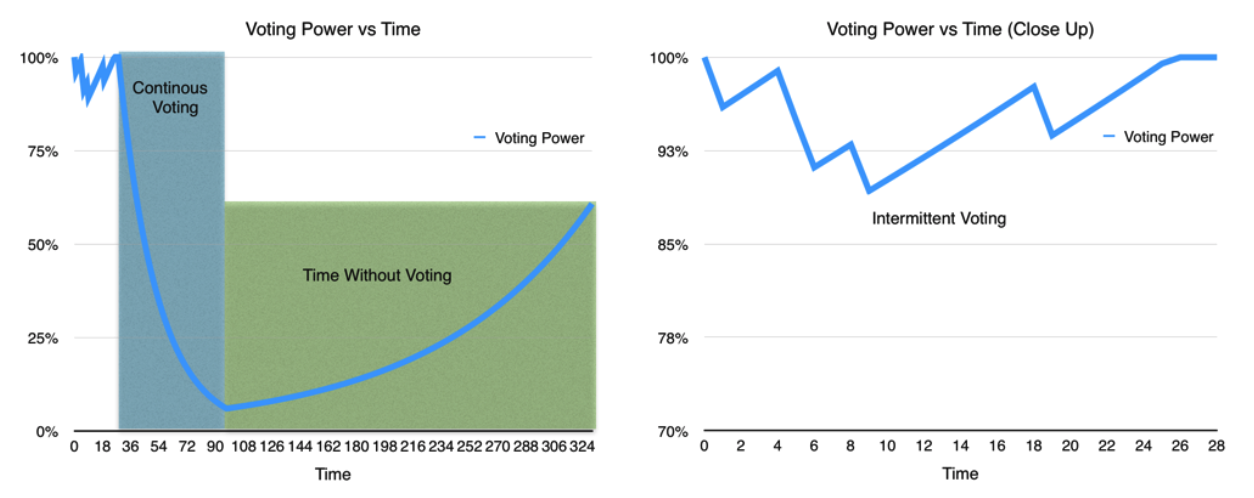
\includegraphics[width=11cm]{img_voting_rate_limiting}

				\paragraph{}
					The charts above shows how a user's voting power decreases every time they vote and then regenerates as time passes without voting. These charts use nominal time unit and could be made to scale to any targeted voting rate. Note that voting power rapidly drops off during periods of continuous voting, and then slowly recovers.
				
				\paragraph{}
					Voting power is multiplied by a user's vesting tokens to determine how much share in the reward pool should be allocated to a given work item.

			\subsubsection{Delayed Payouts}

				\begin{wrapfigure}{r}{0.5\textwidth}
                    \centering
                    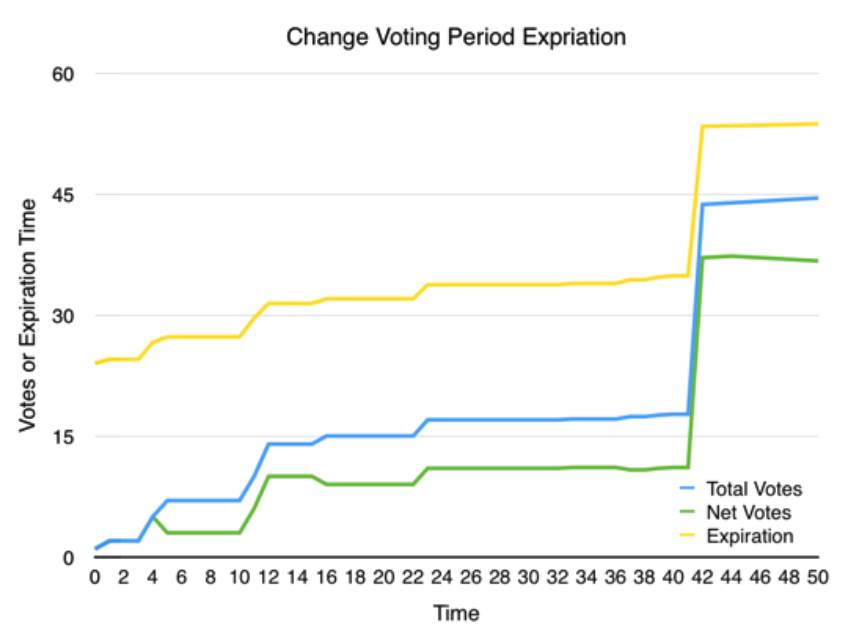
\includegraphics[width=0.5\textwidth]{img_change_voting_period_eg}
                \end{wrapfigure}

				\paragraph{}
					To further prevent abuse, all payouts are delayed a stake-weighted average of 24 hours from the time each vote was cast. This ensures that large stakeholders cannot snipe payouts by voting at the last second before other voters (aka crabs) have a chance to negate the potential abuse. Once a payout is made to the user all votes are reset to 0. If votes come in after the payout then the process begins again.

				\paragraph{}
					This chart shows how the voting period expiration changes in response to new positive and negative votes being applied. New votes extend the payout period in proportion to how large they are relative to all votes that have gone before. Around time 40 a large number of new votes were added which extended the voting period by 12 hours, subsequent smaller votes had far less impact on the voting period.

			\subsubsection{Payout Distribution}

				\begin{wrapfigure}{r}{0.5\textwidth}
					\centering
					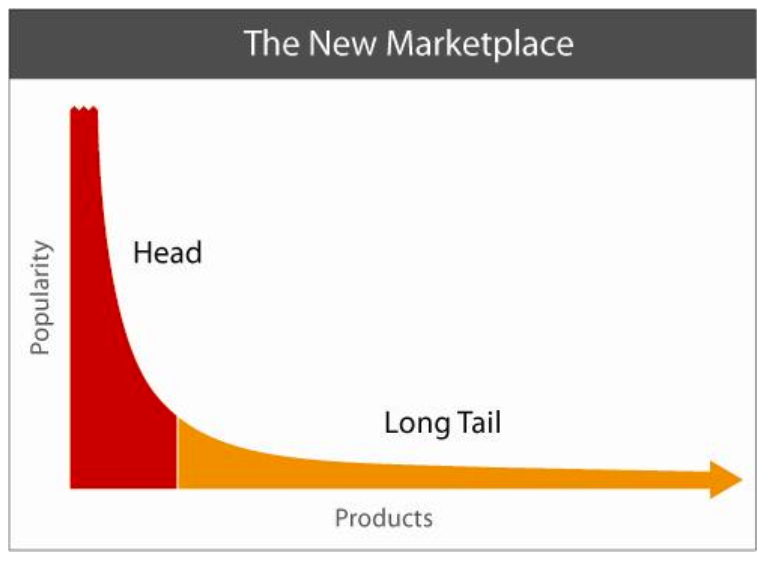
\includegraphics[width=0.5\textwidth]{img_the_new_marketplace}
				\end{wrapfigure}

				\paragraph{}
					One of the primary goals of Steem's reward system is to produce the best discussions on the internet. Each and every year 10\% of the market capitalization of Steem is distributed to users submitting, voting on, and discussing content. At the size of Bitcoin this could be as much as \$1.75 million dollars per day being given to top contributors.

				\paragraph{}
					The actual distribution will depend upon the voting patterns of users, but we suspect that the vast majority of the rewards will be distributed to the most popular content. Steem weighs payouts proportional to n2 the amount of Steem Power voting for a post. In other words, post x would receive a payout proportional to:

				\begin{lstlisting}
		votes[x$]^{2}$ / sum(votes[0...n]$^{2}$)
                \end{lstlisting}

                \paragraph{}
                	Zipf's Law\footnote{Zipf's Law \url{https://en.wikipedia.org/wiki/Zipf\%27s_law}} is one of those empirical rules that characterize a surprising range of real-world phenomena remarkably well. It says that if we order some large collection by size or popularity, the second element in the collection will be about half the measure of the first one, the third one will be about one-third the measure of the first one, and so on. In general, the $k^{th}$-ranked item will measure about 1/k of the first one.

                \paragraph{}
                	Taking popularity as a rough measure of value, then the value of each individual item is given by Zipf's Law. That is, if we have a million items, then the most popular 100 will contribute a third of the total value, the next 10,000 another third, and the remaining 989,900 the  nal third. The value of the collection of n items is proportional to log( n ).

                \paragraph{}
                	The impact of this voting and payout distribution is to offer large bounties for good content while still rewarding smaller players for their long-tail contribution.

                \paragraph{}
                	The economic effect of this is similar to a lottery where people over-estimate their probability of getting votes and thus do more work than the expected value of their reward and thereby maximize the total amount of work performed in service of the community. The fact that everyone "wins something" plays on the same psychology that casinos use to keep people gambling. In other words, small rewards help reinforce the idea that it is possible to earn bigger rewards.

				\subsubsubsection{Rewarding Parent Posts}

					\paragraph{}
						Good discussion requires back and forth posting. When you reply to someone else, they get 50\% of any payout you receive in that thread. This rule applies up to 6 levels deep. Starting a big discussion greatly rewards the parent poster.

					\paragraph{}
						Failure to properly nest your posts in the discussion is a good way to get down voted.

					\paragraph{}
						This incentive structure motivates people to contribute in a way that motivates others to get involved. It encourages people to ask good questions so that others can provide valuable answers.
			\subsubsection{Payouts}

				\paragraph{}
					When a post receives a payout it takes the form of 50\% SMD and 50\% SP. The Steem Power give the user increased voting and transaction power while the SMD gives the user an immediate benefit in a stable currency. As we've already discussed at length, both SP and SMD are designed to encourage long-term holding rather than short-term selling.

	\section{Consensus Algorithm}

		\paragraph{}
			Consensus is the process by which a community comes to a universally recognized, unambiguous agreement on piece of information. There are many algorithms society has developed for reaching consensus about who owns what. Every government on earth is a primitive consensus algorithm whereby the population agrees to abide by a certain set of rules enshrined in a constitution. Governments establish courts, judges, and juries to interpret the subjective facts and render a final decision. Most of the time people abide by the decision even if it was wrong.

		\paragraph{}
			The algorithms used by cryptocurrencies provide a better way to reach consensus. Cryptographically signed testimony from individuals is recorded in a public ledger that establishes the absolute global order of events. A deterministic computer algorithm can then process this ledger to derive a universally accepted conclusion. So long as the members of a community agree on the processing algorithm, the result of the algorithm is authoritative.

		\paragraph{}
			The primary consideration is determining what testimony is allowed to enter the public record. Systems should be designed to minimize the potential for censorship. Censorship on the public ledger is similar to preventing someone from voting in an election. In both cases an individual is prevented from impacting the global consensus.

		\subsection{Consensus in Steem}

			\paragraph{}
				Conceptually, the consensus algorithm adopted by Steem is similar to the consensus algorithm adopted by companies throughout the world. People with a vested interest in the future value of Steem vote to select individuals responsible for including testimony in the public record. Voting is weighted proportional to each individual's vested interest.

			\paragraph{}
				In the world of cryptocurrencies, the public record is commonly referred to as a \textit{blockchain}. A \textit{block} is a group of signed transactions.

			\paragraph{}
				With Steem, block production is done in rounds. Each round 21 witnesses are selected to create and sign blocks of transactions. Nineteen (19) of these witnesses are selected by approval voting, one is selected by a computational proof-of-work, and one is timeshared by every witness that didn't make it into the top 19 proportional to their total votes. The 21 active witnesses are shuffled every round to prevent any one witness from constantly ignoring blocks produced by the same witness placed before.

			\paragraph{}
				This process is designed to provide the best reliability while ensuring that everyone has the potential to participate in block production regardless of whether they are popular enough to get voted to the top. People have three options to overcome censorship by the top 19 elected witnesses: patiently wait in line with everyone else not in the top 19, purchase enough computational power to solve a proof of work faster than others, or purchase more SP to improve voting power. Generally speaking, applying censorship is a good way for elected witnesses to lose their job and therefore, it is unlikely to be a real problem on the Steem network.

			\paragraph{}
				Because the active witnesses are known in advance, Steem is able to schedule witnesses to produce blocks every 3 seconds. Witnesses synchronize their block production via the NTP protocol. A variation of this algorithm has been in use by the BitShares network for over a year where it has been proven to be reliable.

		\subsection{Mining in Steem}

			\paragraph{}
				Traditional proof of work blockchains combine block production with the solving of a proof of work. Because the process of solving a proof of work takes an unpredictable amount of time, the result is unpredictable block production times. Steem aims to have consistent and reliable block production every 3 seconds with almost no potential for forks.

			\paragraph{}
				To achieve this Steem separates block production from solving of proof of work. When a miner solves a proof of work for Steem, they broadcast a transaction containing the work. The next scheduled witness includes the transaction into the blockchain. When the transaction is included the miner is added to the queue of miners scheduled to produce blocks. Each round one miner is popped from the queue and included in the active set of witnesses. The miner gets paid when they produce a block at the time they are scheduled.

			\paragraph{}
				The difficulty of the proof of work doubles every time the queue length grows by 4. Because one miner is popped from the queue every round, and each round takes 21 * 3 = 63 seconds, the dif culty automatically halves if no proof of work is found in no more than 21 * 3 * 4 = 252 seconds.

			\subsubsection{Mining Rewards require Steem Power}

				\paragraph{}
					After the first month, Steem miners are paid in Steem Power (SP). SP is liquidated through the two-year process of "powering down." This means that miners must wait for a long time, likely many months, before sufficient mining rewards have been powered down to allow them to recover the cost of electricity and computational resources. The powering down process discourages creation of mining pools because the pool operator would have to spread payouts over years.

				\paragraph{}
					The effect of paying mining rewards in SP is to prevent miners from using today's price to determine the pro tability of mining. Few people will agree on what the future price will be. This means mining difficulty will be driven by those who place the highest estimate on future value. Miners without a long-term interest in the platform will be discouraged from competing. Ultimately this means that the proceeds of mining are less likely to be dumped on the market because they will accrue to long-term believers in the platform.

			\subsubsection{Mining Algorithm}

				\paragraph{}
					The mining algorithm adopted by Steem requires the miner to have access to the private key of the account that will receive the rewards. This requirement has several important consequences. First it encourages optimization of elliptic curve signature veri cation algorithms needed by Steem. Second it makes it challenging to set up mining pools because the pool operator would have to share control over the reward with all of the "anonymous" miners. Third, it makes it dif cult to use botnets because the botnet operator would have to distribute their private key to all compromised machines.

				\paragraph{}
					The following pseudocode describes how the proof-of-work hash value is calculated:

				\begin{lstlisting}
Let H	= Head Block ID
Let H2	= SHA256(H+NONCE)
Let PRI	= Producer Private Key
Let PUB	= Producer Public Key
Let S	= SIGN(PRI, SHA256( H ) )
Let K	= RECOVER_PUBLIC_KEY( H2, S )
Let POW	= SHA256( K )
				\end{lstlisting}

			\subsubsection{Botnet Resistant}

				\paragraph{}
					Many proof of work coins end up being mined by botnets. A botnet is a collection of thousands or millions of machines that have been compromised by hackers. These hackers steal the computational and electrical resources of compromised machines to mine cryptocurrency tokens.

				\paragraph{}
					Steem has many properties that prevent these computational thieves from profiting. Botnet operators are profit seeking enterprises and typically sell their stolen resources to the highest bidder. This means that those who utilize a botnet pay for the computational power in the same way that someone who uses Amazon EC2 does. The vesting requirement of Steem means that the capital spent on buying the resources of the botnet will be tied up for a long period of time during which the operator is exposed to price volatility.

				\paragraph{}
					Another way that botnet operators are prevented from profiting is the requirement to distribute the private key to all compromised machines. If even one compromised computer is discovered, the operator could lose their coins.

				\paragraph{}
					The last mitigation is the dependency on latency. Most botnets are comprised of computers with poor internet connections, these slow Internet connections will dramatically reduce the effectiveness of the computational resource.

				\paragraph{}
					It should be more pro table and less risky for botnet operators to use their resources for other activities than mining STEEM.

			\subsubsection{Mining Pool Resistant}

				\paragraph{}
					Miners have a total of 3 seconds to receive a block, solve the proof of work, and get the transaction to the next block producer. Much of this time will consist of network latency which means that it is critical for miners to be well connected to the network to make the most effective use of their computational resources.

				\paragraph{}
					Because of the constantly changing head block and network latency, forwarding a template for mining a specific block to participants of a mining pool adds additional network latency and reduces efficiency of pooled mining significantly.

	\section{Eliminating Transaction Fees}

		\paragraph{}
			Steem goes to great lengths to reward people for contributing to the network. It would be counterproductive to turn around and charge people every time they attempt to interact with the community.

		\paragraph{}
			Blockchain technology currently depends upon transaction fees to prevent spam. These fees suffer all of the known problems with microtransactions and prevent blockchains from being used for low-value transactions. Truly decentralized applications must offer users the appearance of free transactions if they wish to compete with their centralized alternatives. This paper outlines the approach used by Steem to eliminate the need for fees and thereby enable a wide range of previously untenable decentralized applications.

		\subsection{The Problem With Fees}

			\paragraph{}
				Blockchains are decentralized networks where all transactions are broadcast to all peers. Every so often a block is produced that includes some or all of the pending transactions. All blockchains must find a solution to prevent malicious users from consuming all of the available network capacity with worthless transactions. These worthless transactions can prevent other valuable transactions from being processed and ultimately destroy the network.

			\paragraph{}
				The solution adopted by most blockchains thus far is to charge a minimum transaction fee. A fee worth just a few cents is enough to make attacking the network expensive and unprofitable. While this approach solves the spam problem, it introduces new problems. Imagine solving the email spam problem by introducing a small fee on every email; people wouldn't use email.

			\subsubsection{Micropayments Don't Work}

				\paragraph{}
					The fundamental problem with charging transaction fees is that micropayments don't work, especially for low-value user actions. When a fee is charged on every transaction, it limits the types of transactions that a decentralized network can process. Regardless of how rational the argument for the necessity of fees, users still hate the experience of being nickeled and dimed for everything that they do.

				\paragraph{}
					Imagine if the websites we use every day charged us a fee every time we modify our accounts by changing the password. Users expect certain things to be free. Requiring users to make a decision on whether or not an action is worth a small fee creates anxiety that causes users to leave.

				\begin{quote}
						A transaction can't be worth so much as to require a decision but worth so little that that decision is automatic. There is a certain amount of anxiety involved in any decision to buy, no matter how small, and it derives not from the interface used or the time required, but from the very act of deciding.\\

						Micropayments, like all payments, require a comparison: "Is this much of X worth that much of Y?" There is a minimum mental transaction cost created by this fact that cannot be optimized away, because the only transaction a user will be willing to approve with no thought will be one that costs them nothing, which is no transaction at all.

						- Clay Shirky\protect\footnote{Clay Shirky, The Case Against Micropayments\newline\url{http://www.openp2p.com/pub/a/p2p/2000/12/19/micropayments.html}}\\
				\end{quote}

				\paragraph{}
					In the world of financial payments, small fees are acceptable because the value of the transaction is extremely high relative to the fee charged, and the buyer has already made a decision to buy. The world of potential blockchain applications is far greater than just financial payments and includes many necessary transactions for which fees are simply unacceptable to users.

				\paragraph{}
					Systems like BitShares, Nxt, Ripple, Counter Party and Stellar all allow users to place limit orders on the blockchain and all of them charge users a small fee to perform this action. Later if the user wishes to cancel their order, another fee is charged. Systems like Ethereum take micropayments to a whole new level: charging per calculation. All of these systems struggle to attract new mainstream users for the same reasons that a decentralized search engine would struggle to attract users from Google if it charged a small fee for every search. It doesn't matter how good the service is, people expect certain things to be free. This is true even if a user ends up paying more overall under a different fee structure.

			\subsubsection{Fees are a Barrier to Entry}

				\paragraph{}
					Any fee creates a barrier to entry for new users. Before someone can experiment with Ethereum they must acquire some ETH tokens. Anyone wanting to build a decentralized application on Ethereum must pass on the cost to their customers. Buying a crypto currency is not an easy task and rarely makes sense for amounts less than \$10. This means that new users wanting to try out a new decentralized application must first be convinced to part with \$10.

			\subsubsection{Changing Fees}

				\paragraph{}
					Over time a network must adjust fees. This can happen either due to an increase in the value of the token or due to a surge in capacity. Users like predictable fees and guaranteed service. While it is possible to dynamically adjust fees during times of heavy use, the result is a poor user experience.

			\subsubsection{Sybil Attacks}

				\paragraph{}
					Centralized websites prevent spam through rate limiting and some form of ID veri cation. Even something as simple as reCAPTCHA\footnote{reCAPTCHA, Easy on Humans, Hard on Bots\newline\url{https://www.google.com/recaptcha/intro/index.html}} is sufficient to limit the creation of fake accounts. If someone abuses their account then centralized websites are free to block the account.

				\paragraph{}
					In a decentralized system there is no direct way to ban users nor centralized provider able to host a reCAPTCHA and enforce rate limiting of accounts. In fact, the inability to censor users is one of the main selling points of blockchain technology.

			\subsubsection{Full Reserve vs Fractional Reserve}

				\paragraph{}
					Let's view a blockchain like an Internet Service Provider (ISP) co-op which owns all of the cables in the town and has a maximum amount of bandwidth that it can provide at any time. People living in the town can buy shares in the ISP and in exchange they are entitled to utilize a portion of the available bandwidth.

				\paragraph{}
					The ISP has two choices, run a "full reserve" or "fractional reserve" system. Under a full reserve system each user is only allowed a fraction of the maximum bandwidth proportional to her shares. Because not everyone uses the Internet at the same time, the town's network would be significantly underutilized.

				\paragraph{}
					Under a fractional reserve system the individual users could utilize more bandwidth than they are entitled to at any given point in time so long as not everyone uses the Internet at the same time. The problem with operating a fractional reserve is that congestion occurs anytime too many people wish to use the network at the same time. The ISP needs a way to prioritize bandwidth during congested periods. In the most extreme case, a fully congested network must revert to a full reserve system. The challenge is setting the proper fractional reserve ratio.

		%Note, this sub section is missing from the original doc contents
		\subsection{Bandwidth Instead of Micropayment Channels}

			\paragraph{}
				The solution to the problems with micropayments is in implementing \textit{dynamic fractional reserves}. Under this model the blockchain will automatically adjust the reserve ratio for the network during times of congestion. The blockchain will set a target utilization that leaves enough headroom for short term surges in demand. Any time the surges are sustained the blockchain reduces the maximum bandwidth-per-share. When a surge is over and there is surplus capacity the blockchain can slowly increase the bandwidth-per-share.

			\paragraph{}
				Bandwidth used by an individual user should be measured over a suitably long period of time to allow that user to time-shift their usage. Users tend to login, do many things at once, then logout. This means that their bandwidth over a short period of time may appear much higher than if viewed over a longer period of time. If the time window is stretched too far then the reserve ratio will not adjust fast enough to respond to short-term surges, if the window is too short then clustering usage will have too big of an impact on normal users.

			\paragraph{}
				In our estimate it should be sufficient to measure the average weekly bandwidth usage of users. Every time a user signs a transaction, that transaction is factored into their own individual moving average. Any time a user's moving average exceeds the current network limit their transaction is delayed until their average falls below the limit.

			\subsubsection{Example Implementation}

				\paragraph{}
					Let B equal a user's average bandwidth at time T. Let W equal the number of seconds per week, and let N equal the size of the new transaction that occurred S seconds after T. Given this information the blockchain can calculate the new average bandwidth for a user as:

				\begin{lstlisting}
Bnew = MIN(0,B * (W-S) / W) + N * S / W
Tnew = T + S
				\end{lstlisting}

				\paragraph{}
					Each user is entitled to an average weekly bandwidth of:

				\begin{lstlisting}
Let U = the user's SP
Let S = the total number of SP
Let R = the current reserve ratio between 1 and Rmax
Let C = the maximum block size capacity set by witnesses
Let L = the total blocks per week
Let M = C * L * R
Allocation= M * U / S
				\end{lstlisting}

				\paragraph{}
					A user would be entitled to an average bandwidth of M * U / S. Any time a transaction would cause the user's average to go above this threshold they would be unable to transact until enough time passes to lower the average.

				\paragraph{}
					The network can increase the reserve ratio, anytime blocks are less than half the target capacity and decrease it anytime they are more than half. The algorithm used to adjust R is designed to react quickly to decrease the reserve ratio when there is a surge in demand, while acting slowly to increase the reserve ratio in period of low demand.

				\paragraph{}
					The minimum reserve ratio is 1, and the maximum reserve ratio should be calculated to prevent small stakeholders from consuming all of the available bandwidth. If no one is using the available bandwidth then the reserve ratio can grow until a user with just 1 satoshi of the currency is able to transact every single block.

			\subsubsection{Case Study: Bitcoin}

				\paragraph{}
					To understand how this algorithm would work on Bitcoin it is necessary to estimate a reasonable value for the reserve ratio, R, based on actual usage. Based upon the total supply of 15M BTC and a daily transaction volume of 400K BTC\footnote{Bitcoin Estimated Transaction Volume\newline\url{https://blockchain.info/charts/estimated-transaction-volume?showD}}, we can derive a minimum reserve ratio of 38 for Bitcoin. Using the equations we can calculate the weekly bandwidth (in bytes) allowed per BTC to be:

				\begin{lstlisting}
Let C = 1MB = 1024*1024
Let L = 1008 (blocks per week)
Let R = 38
Let S = 14000000 BTC (supply minus Satoshi's unmoving coins)
Let U = 1 BTC
CLR/S = 2869 bytes per week, or about 5 transactions/week per BTC
				\end{lstlisting}

				\paragraph{}
					Since R = 38 is a lower bound on the reserve ratio, CLR/S is a lower bound on the permitted bandwidth. This simple case study suggests a user will require at most 0.20 BTC (over \$80 as ofthiswriting)totransactonceperweek. However,thisisalooseupperboundderivedfrom the assumption that all BTC are equally mobile. This is not the case -- users with dozens or hundreds of bitcoins do not necessarily transact dozens or hundreds of times a week! The "leftover" transactions that those users "should" have made will increase the reserve ratio, allowing their unused bandwidth to be "recycled" for smaller users.

				% TOOD : insert extra spacing or horizontal rule

				\paragraph{}
					All of the above estimates are conservative upper bounds assuming coins and usage are distributed in a relatively flat manner. The reality is that heavy users, such as exchanges, have a much higher coin-to-usage ratio than lighter users, which in turn means that actual minimum balance requirements are far lower.

				\subsubsubsection{Impact of Capacity}

					\paragraph{}
						Blockchain capacity isn't necessarily capped. It is well within the technological capability of internet infrastructure to increase the Bitcoin block size to 10MB which in turn will reduce the minimum required balance by a factor of 10. While Bitcoin currently supports about 3 transactions per second, alternative implementations are capable of over 1000 transactions per second. This changes our conservative upper bound to 0.0006 BTC or about \$0.25, meaning that an account holding \$0.25 would be able to transact at least once per week on average (and likely many more times because we're dealing with a fairly loose upper bound).

				\subsubsubsection{Maximum Number of Unique Users}

					\paragraph{}
						We can use similar math to calculate the maximum number of unique users that the network can allow to transact once per week as: B*W/T. T represents the average transaction size. This means Bitcoin could support about 2 million users transacting once per week assuming each user had an equal balance.

				\subsubsubsection{Comparison to Fees}

					\paragraph{}
						If we assume a user with \$25 dollars worth of BTC transacts once per week and pays a \$0.04 cent fee each time then they would pay over \$2.00 in fees per year. A user would have to earn a 8\% rate of return on their \$25 dollars just to break even with paying fees. Chances are that users were going to hold their money on the blockchain anyway, so this user with \$25 worth of BTC just saved \$2 over the course of a year by adopting a rate-limiting approach rather than a fee-based approach. With just \$175 they could transact every single day and save \$14 per year.

			\subsubsection{Account Creation}

				\paragraph{}
					Steem's account-based system with publicly known balances simpli es the implementation of the bandwidth-based rate limiting algorithm. Any account with a balance below the minimum required to transact once per week would be unable to transact. This implies that all new accounts should be funded with at least this minimum balance. It also implies that users wishing to transact in smaller amounts can, so long as they hold a larger balance and reuse the account.

				\paragraph{}
					It is possible for a low-balance account created during a time of low usage to become inaccessible if the network usage picks up. The funds could be recovered at any time by transferring a larger balance into the account.

				\paragraph{}
					In order to maintain a reasonable user experience with a minimum number of hung accounts, all new accounts should start out with a balance 10 times the minimum required to transact weekly. This way even if demand increases by a factor of 10 the account will remain viable.

				\paragraph{}
					Any initial account balance would have to come from the user creating the account and not from token creation due to the potential for sybil attacks.

			\subsubsection{Justifying Minimum Balances}

				\paragraph{}
					The concept of forcing users to maintain a minimum balance flows naturally from the value of a user\footnote{Forbes, Tristan Louis, "How Much is a User Worth?"\newline\url{http://www.forbes.com/sites/tristanlouis/2013/08/31/how-much-is-a-us}}. Anyone running a business knows that every single user has significant value. Businesses spend anywhere from \$30 to \$200 to acquire a user. Sometimes they pay users directly, other times they pay for advertizing, and still other times entire companies are bought just for their user base. After a company acquires a user they often given them many \textit{free services} just to keep them around long enough to monetize them through some other means.

				\paragraph{}
					Ripple uses a minimum balance\footnote{Ripple, Account Reserves\newline\url{https://ripple.com/build/reserves/}} that scales with account resource use and requires that new accounts get funded with at least this minimum balance. Currently this minimum balance is about \$0.15 which is greater than the \$0.10 we estimated would allow someone to transact freely at least once per week.

				\paragraph{}
					A blockchain can enforce a minimum value per user through the simple process of requiring a minimum balance. Any business that wishes to bring a new customer to the blockchain can pre-fund that user's account with the minimum balance that would allow them to transact. Requiring a relatively large fee (\$1.00) to sign up new users will naturally force anyone offering free accounts to vet the quality and uniqueness of each account before registering them with the blockchain.

				\paragraph{}
					Maintaining a minimum balance is effectively the same as making users pay transaction fees with the interest they could have earned on their balance. The minimum balance is simply the balance required to earn enough interest to pay a fee in a relatively short period of time.

				\paragraph{}
					Fortunately, the minimum balance required can be as low as a dollar and this is something users can understand and appreciate. The opportunity cost of lost interest doesn't incur the cognitive cost of a micro-fee and is far more acceptable to users.

				\paragraph{}
					The STEEM used to pre-fund an account is Powered Up in the new account (i.e., converted to Steem Power).

			\subsubsection{Adjusting the Reserve Ratio}

				\paragraph{}
					Rate limiting requires that the network adjust the reserve ratio quickly enough to mitigate the impact of an attacker attempting to  ood the network. Let's assume the attacker has a large balance, say 1\% of the available tokens. If we also assume that the network targets 50\% utilization, then a sustained attack should  nd this user throttled to 25\% of network capacity assuming everyone else is also using 25\% of the capacity. Stated another way, the largest single user should never be able to consume more than 50\% of the target capacity unless they own more than 50\% of the SP.

				\paragraph{}
					Let's use an initial reserve ratio of 200x. Due to fractional reserves, this means someone holding 1\% of the tokens has the right to demand transactions totalling 2x the maximum block size. In order to bring the network usage of the attacker down to 25\% the reserve ratio would have to fall to 25x. This would cause the minimum balance required to transact once per week to grow by 8x.

				\paragraph{}
					The blockchain can establish a response rate that says any sustained increase in usage should be brought down to the target capacity in within a short period of time (say 30 seconds). An attacker attempting to spam the network shouldn't be able to disrupt service for normal users for more than a minute.

				\paragraph{}
					While reductions in the reserve ratio must be quick and non-linear to counter abuse, increases in the reserve ratio should be slow and linear. If the network adjusted in both directions in just 30 seconds then an attacker could pulse the network. A flood of transactions should be corrected in 30 seconds and then take a hour to return to their pre-attack levels. Under this model the attacker could flood the network for 30 seconds per hour or less than 1\% of the time.

				\paragraph{}
					There must be a slow constant upward pressure on the reserve ratio any time network usage is below 50\% until the network hits the maximum reserve ratio. The maximum reserve ratio determines the minimum required stake to flood the network in short bursts.

				\paragraph{}
					Any user with fewer than TOTAL\_TOKENS / (2*RESERVE\_RATIO) will be unable to produce enough transactions to fill even a single block. With a reserve ratio of 200, this means any user with less than 0.25\% of the currency cannot create enough transactions to delay anyone's service.

			\subsubsection{Effectiveness Relative to Fees}

				\paragraph{}
					To compare the effectiveness of rate limiting to fees we must consider how the two systems react to intentional network flooding by an attacker. Under Bitcoin an attacker with \$10,000 dollars could disrupt service for an entire day by filling every single block. The same attacker would be unable to disrupt service for even a single block under the dynamic fractional reserve rate limiting approach.

				\paragraph{}
					If we go to a more extreme case and assume the attacker holds 1\% of all coins then we presume an attacker with \$60 million dollars. Such an attacker could deny the Bitcoin blockchain service for 16 years unless the miners increased fees or capacity. Even if fees were raised to \$15 per transaction, the attacker could still keep the network flooded for 16 days.

				\paragraph{}
					Under the rate limiting approach, someone who holds 1\% of all coins with an intent to flood the network would achieve their goal for less than 30 seconds.

			\subsubsection{Renting vs. Buying vs. Time Sharing}

				\paragraph{}
					When someone owns a house they expect the right to use the house for free. If a group of people buy a house together then each can expect the right to use the house proportional to their percentage ownership in the house. A fee based blockchain is like renting the house from its owners, whereas rate limiting is like a timeshare among owners.

				\paragraph{}
					If a house is owned by multiple people then those individuals must decide how they wish to timeshare the house. Someone who owns 50\% of the house but only uses it one weekend per year might expect to be paid by the individuals who take their unused time. This is the mindset of a fee based system.

				\paragraph{}
					On the other hand, someone who owns 50\% of the house is speculating that demand for the house will increase in the future and they will be able to sell their stake for more. Any owner who owns more of a house than they use becomes a real estate speculator. With this mindset rather than collecting rent, they collect appreciation.

				\paragraph{}
					The value of a share is derived from how much time it can potentially grant its owner. Owning 1\% of a house and getting it 1 weekend per year is the lowest value of a share. However, if half of the shareholders never use their weekend, then the value per timeshare rises to 2 weekends per year. If those inactive users instead opt to rent their unused time, then it falls back to 1 weekend per year. If those unused timeshares were sold to people who would use them then the value of a timeshare would fall by 50\%. Unless the rent collected is greater than the fall in share value the timeshare owners are making an economic miscalculation.

				\paragraph{}
					Using this rationale we can assume that a system based on fees will either be more expensive for its users or be less profitable for its collective owners. An individual small owner may profit by renting out his small time slice, but only at the expense of all other timeshare owners. In effect, the cost of the falling timeshare value is shared among all owners whereas the pro ts are centralized in the single owner who decided to rent his share.

				\paragraph{}
					We can conclude from this that a blockchain is best served by not using usage fees at all. If a usage fee were to be charged as an alternative to rate limiting, then it should be the equivalent of buying enough timeshares and committing to hold them long enough to gain the right use it once.

				\paragraph{}
					Stated another way, a transaction fee should be equal to the minimum account balance necessary to transact once per week and it should be refunded at the end of the week. Assume the minimum account balance is \$1 and allows someone to transact once per week. If someone with a \$1 balance that wishes to perform 5 transactions at once they will have to increase their balance to \$5 for a week either before or after their transactions.

				\paragraph{}
					In theory a market could form where users can borrow the stake required. In practice it is more ef cient for users to simply buy and sell the timeshares necessary to meet their desired usage rate. In other words, the cost of negotiating micro-loans is greater than the cost of maintaining a balance suitable for your maximum weekly usage.

				\paragraph{}
					Decentralized rate limiting of transactions can enable new types of decentralized applications that were not viable when every use of the application required a micropayment. This new model gives application developers the ability to decide if and when to charge their users for transactions.

	\section{Performance and Scalability}

		\paragraph{}
			The Steem network is built upon Graphene, the same technology that powers BitShares. Graphene has been publicly demonstrated sustaining over 1000 transactions per second on a distributed test network. Graphene can easily scale to 10,000 or more transactions per second with relatively straightforward improvements to server capacity and communication protocols.

		\subsection{Reddit Scale}

			\paragraph{}
				Steem is capable of handling a larger userbase than Reddit. In 2015 Reddit's 8.7 million users generated an average of 23 comments per second\footnote{Reddit Statistics, Number of Users and Comments per Second\newline\url{http://expandedramblings.com/index.php/reddit-stats/2/}}, with an average of 83 comments per year per user. There were 73 million top-level posts, for an average of 2 new posts per second. There were about 7 billion up votes creating an average voting rate of 220 votes per second. All told, if Reddit were operating on a blockchain it would require an average of 250 transactions per second.

			\paragraph{}
				To achieve this industry-leading performance, Steem has borrowed lessons learned from the LMAX Exchange\footnote{Martin Fowler, The LMAX Architecture\newline\url{http://martinfowler.com/articles/lmax.html}}, which is able to process 6 million transactions per second. Among these lessons are the following key points:

			\begin{enumerate}
				\item Keep everything in memory.
				\item Keep the core business logic in a single thread.
				\item Keep cryptographic operations (hashes and signatures) out of the core business logic.
				\item Divide validation into state-dependent and state-independent checks.
				\item Use an object oriented data model.
			\end{enumerate}

			\paragraph{}
				By following these simple rules, Steem is able to process 10,000 transactions per second without any significant effort devoted to optimization.

			\paragraph{}
				Keeping everything in memory is increasingly viable given the recent introduction of Optane\texttrademark technology from Intel\footnote{Introducing Intel Optane Technology - Bringing 3D XPoint Memory to Storage and Memory Products\newline\url{https://newsroom.intel.com/press-kits/introducing-intel-optane-technology-bringing-3d-xpoint-memory-to-storage-and-memory-products/}}. It should be possible for commodity hardware to handle all of the business logic associated with Steem in a single thread with all posts kept in memory for rapid indexing. Even Google keeps their index of the entire internet in RAM. The use of blockchain technology makes it trivial to replicate the database to many machines to prevent loss of data. As Optane\texttrademark technology takes over, RAM will become even faster while gaining persistence. In other words, Steem is designed for the architectures of the future and is designed to scale.

	\section{Allocation \& Supply}

		\paragraph{}
			The Steem network starts with a currency supply of 0 and allocates STEEM via proof of work at a rate of approximately 40 STEEM per minute to miners, with an additional 40 STEEM per minute being created to seed the content and curation reward pools (for a total of 80 STEEM per minute). Then the network starts rewarding users who convert to SP. At this point, STEEM grows at a rate of approximately 800 STEEM per minute due to the combined effects of the various Contribution Rewards summarized below:

		\paragraph{}
			\textbf{Contribution Rewards:}

		\begin{itemize}
			\item Curation rewards: 1 STEEM per block or 3.875\% per year, whichever is greater
			\item Content Creation rewards: 1 STEEM per block or 3.875\% per year, whichever is greater
			\item Block production rewards: 1 STEEM per block or 0.750\% per year, whichever is greater
			\item POW inclusion rewards before block 864,000: 1 STEEM per block (awarded as 21 STEEM per round)
			\item POW inclusion rewards after block 864,000: 0.0476 STEEM per block (awarded as 1 STEEM per round) or 0.750\% per year, whichever is greater.
			\item Liquidity rewards: 1 STEEM per block (awarded as 1200 STEEM per hour) or 0.750\% per year, whichever is greater
		\end{itemize}

		\paragraph{}
			\textbf{Power Rewards:}

		\begin{itemize}
			\item Steem Power rewards: For each STEEM created by the above rewards, 9 STEEM are divided among all Steem Power holders.
		\end{itemize}

		\paragraph{}
			\textbf{SMD operations:}

		\begin{itemize}
			\item SMDrewards: A percentage of SMD value is created at an APR set by the witnesses and paid to SMD holders as SMD
			\item Feed Rate following: The amount of STEEM for which the total SMD in existence can be redeemed will change based on changes in the price feed. This change is effectively destruction ("burning") of STEEM when the value of STEEM (as measured by the feed) is increasing, or creation of STEEM when the value of STEEM (as measured by the feed) is declining.
		\end{itemize}

		\paragraph{}
			The percentage constraints effectively ensure the incentives for rewards do not become meaninglessly small over time, which is intended to prevent the system from experiencing the "speed bump" in the growth pattern of many other blockchains, where an initial growth spurt fueled by high incentives for early participants is followed by prolonged stagnation as the continually falling incentives drop below the level necessary to induce newcomers to join.

		\paragraph{}
			The overall effect of these percentage constants on allocation and supply is that the (approximately) 800 STEEM per minute rate remains in effect for some time (i.e. units of STEEM), but drops in percentage terms (i.e., 800 STEEM is a smaller and smaller fraction of the total supply as the total supply grows larger and larger). When the various individual components of the 800 STEEM per minute rate reach their respective percentage-based floors, each floor halts the fall in its component of the rate. This in turn means that, over the long term, the nominal rate will rise from 800 STEEM per minute to the (time-varying, supply-dependent) value needed to maintain a constant annualized growth rate of 10\% for the Contribution Incentives, and a constant annualized growth rate of 100\% for the combined effect of the Contribution Incentives and the Power Incentives. The overall effect is a doubling of the STEEM supply each year (but, as detailed in the next section, if most users Power Up then much of this doubling is effectively a "split" which does not transfer ownership).

		\paragraph{}
			The overall supply picture is complicated by the effect of SMD operations, which may result in large-scale creation or destruction of STEEM through feed rate following and SMD rewards, as discussed in the SMD section. Other, smaller-scale complicating effects also exist, including unclaimed incentives (e.g. block rewards for missed blocks), noise due to miner luck in proof-of-work production, and the effects of changes in the miner queue length due to a change in the network's total hashpower.

		\subsection{Impact of Token Creation Rate}

			\paragraph{}
				At first glance, 100\% annual increase in the STEEM supply may appear to be hyper-in ationary and unsustainable. Those who follow the Quantity Theory of Money\footnote{Quantity Theory of Money,\newline\url{http://www.investopedia.com/articles/05/010705.asp}} may even conclude that the value of STEEM must fall by approximately 5.6\% per month. We know from countless real-world examples that the quantity of money does not have a direct and immediate impact on its value, though it certainly plays a role.

			\paragraph{}
				Because 90\% of all STEEM created is distributed back to holders of SP, the result is similar to having a 2:1 "split" every year rather true inflation. The total rate of expenditures used to reward contributors is about 10\% of the market capitalization per year, a rate well below what Bitcoin sustained for the first 7 years after it launched.

			\paragraph{}
				Creating new STEEM to pay an incentive to a particular user or group has a negative effect on every other user's balance in terms of their percentage of the STEEM supply. If exactly 90\% of the STEEM supply is held in SP, then the negative effect of Contribution Incentives on SP holders' balances is exactly balanced by the positive effect of Power Incentives; SP holders get more STEEM (in nominal terms) but their percentage of the chain (in terms of fraction of the total supply) is unchanged. If less (more) than 90\% of the STEEM supply is held as SP, the two effects still point in opposite directions, but the positive (negative) effect becomes greater and the sum of these two effects will tend to pull the SP balance toward 90\%. This "pull" does not mean that the SP value must hold at 90\% over the long term, because incentive recipients will (and in some cases must) put their STEEM in SP, which means the "pull" towards 90\% is not the only force on the percentage of STEEM supply held as SP.

			\paragraph{}
				From August 2008 through January 2009 the U.S. money supply\footnote{United States Money Supply, 2009\newline\url{https://research.stlouisfed.org/fred2/graph/?s\%5B1\%5D\%5Bid\%5D=AMBNS}} grew from \$871B to \$1,737B, a rate of over 100\% per year and then continued to grow at about 20\% per year for the next 6 years. All told the money supply in the U.S. has grown by 4.59x over less than 7 years. During that same time, the value of the dollar relative to goods and services has fallen less than 10\% according to the government's price index\footnote{CPI Inflation Index, United States Dollar 2008-2016\newline\url{http://data.bls.gov/cgi-bin/cpicalc.pl?cost1=1&year1=2008&year2=2016}}. This real-world example demonstrates that supply is only one component of price.

			\paragraph{}
				The price of a digital commodity, like STEEM, is driven by both supply and demand. If new STEEM is allocated to those who are holding long-term then the increase in supply is offset by the corresponding demand to hold. The impact of this change in supply is postponed until a future date when the long-term holder decides to sell. The sell pressure is then distributed over 2 years.

			\paragraph{}
				When a long-term holder decides to exit, the supply of STEEM on the market will increase and push the price down. This downward pressure is countered when a new long-term holder decides to buy up the STEEM and convert it back into SP. We can therefore conclude that the price will mostly be impacted by a change in demand for holding STEEM long-term.

			\paragraph{}
				Of the 100\% annual increase in the virtual STEEM supply, 5\% of it is in the form of Steem Dollars (SMD). SMD represents a commitment to create a dollar's worth of STEEM in the future and does not impact the amount of STEEM on the market today. The change in debt-to-ownership ratio may impact the perceived value of STEEM, but it does not map directly into a fall in the value of STEEM. If the value of Steem rises over time, then the amount of STEEM that may be created in the future will be less and the corresponding "in ation" never actually happened.

			\paragraph{}
				All told the total "spending" Steem does to fund content, curation, mining, and liquidity rewards amounts to just 10\% APR or 1.2\% per month. The same wealth transfer could be implemented without any change in the STEEM supply by implementing a negative interest rate on liquid STEEM of around 10\% per month. Stated another way, it could be implemented by charging a 3\% fee (similar to credit cards) on every transfer and having 1\% of all STEEM transferred every single day. The Bitcoin network transfers\footnote{Bitcoin Transaction Volume\newline\url{https://blockchain.info/charts/estimated-transaction-volume}} 400,000 BTC out of 15.5M (or 2.5\% daily).

			\paragraph{}
				The purpose of liquid STEEM is to facilitate changes in ownership between long-term holders. It is this change in ownership that the network "taxes" to fund growth. This transfer tax can be avoided almost completely by automatically selling STEEM for SMD every week as the network converts SP back to STEEM. The total time spent holding STEEM will be so small that any impact of changing STEEM supply will be insigni cant next to volatility and other market fees.

			\subsubsection{Impact of Token Creation Rate Greater than Ninety-Percent}

				\paragraph{}
					As of May 1, 2016, over 98.49\% of all STEEM has been converted to SP. This demonstrates that demand to hold long term dominates. In this environment both liquid STEEM and SP are diluted to fund rewards.

				\paragraph{}
					For the first 2 years of Bitcoin's life the network sustained an annual in ation rate\footnote{Bitcoin Annual In ation Rate, Bitcoin Talk Forum\newline\url{https://bitcointalk.org/index.php?topic=130619.0}} of over 100\%. For the first 5 years it was over 30\%, and for the first 8 years it was over 10\%. According to the tool for estimating future in ation included with the Steem source code, Steem by contrast will achieve an instantaneous annual rate of approximately 12\% after just 1 year (not including the effects of SMD operations).

			\subsubsection{Accounting In Steem}

				\paragraph{}
					The increase in the supply of STEEM is mostly an accounting artifact created by the desire to avoid charging negative interest rates on liquid STEEM. Negative interest rates would complicate the lives of exchanges which would have to adjust user balances to account for the negative rate of return of STEEM held on deposit. Mirroring the blockchain logic exactly would be error prone and complicate integration and adoption. Therefore, STEEM has chosen to never charge someone's account, but instead to increase supply. This achieves a similar economic result without forcing everyone accepting STEEM deposits to implement negative interest rates on their internal ledger.

				\paragraph{}
					A side effect of increasing the supply is that the network will require ever increasing levels of precision in its accounting. On average the number of bits required to represent a typical account will grow by 1.3 per year. It will only take 10 years before numbers involved no longer fit within the 53 bit precision supported by JavaScript or the 64 bit precision supported by CPUs. Over time the magnitude of the numbers involved grows beyond human scale and comprehension; furthermore, the least significant bits have so little economic value as to render them meaningless.

				\paragraph{}
					In order to compensate for the ever increasing precision, the STEEM network performs a 10:1 "reverse split" every 32,000,000 blocks (about 3 years). At this point in time all balances of STEEM are divided by 10 and all prices are multiplied by 10. Cryptocurrency exchanges will have to suspend trading around this time and update the account balances and price history to reflect the "reverse split" before resuming trading.

				\paragraph{}
					All rounding errors will be in favor of the network. Every balance may lose up to 0.009 STEEM due to rounding, but this amount of STEEM should be economically insignificant. Collectively all holders of SP will lose at most 0.009 STEEM.

	\section{The Power of Steem}

		\paragraph{}
			Steem recognizes that the value of all user contributions (posts and votes) is greater than the sum of the parts. A single comment is worth next to nothing, but millions of curated posts is worth many millions (or possibly even billions) of dollars. A single vote provides little curation value, but billions of votes is very effective curation. Content without curation is of limited value. Given all the content of the Internet minus the links between it, Google would struggle to produce useful search results. It is the links between information that give it significant value.

		\paragraph{}
			Because everyone benefits, everyone should pay. In other words, no individual user should be expected to pay for anything, but instead should be paid for everything they do that brings value to Steem. All we need to do is ascertain which user contributions bring a social network value and which ones don't.

		\paragraph{}
			Collectively Reddit users vote 220 times per second and make 23 posts per second. Reddit is valued between \$500 million\footnote{Reddit Valuaton, Newsweek, 2014\newline\url{http://www.newsweek.com/investors-think-reddit-worth-500-million-26}} and \$4 billion\footnote{Worth of Web, March 2016\newline\url{http://www.worthofweb.com/website-value/reddit.com/}} which means that each and every upvote and post is worth between \$0.06 and \$0.50 assuming the value of Reddit is mostly within the past year's worth of activity. One could argue that most of the value of Reddit is the near-real-time discussions that have occurred within the past week which would dramatically increase the value of new activity. People go where people are today, not where people were last year.

		\subsection{No Micropayments, Tips Optional}

			\paragraph{}
				Existing attempts at integrating a cryptocurrency into a social media platform have focused on enabling users to pay one another. Many services have attempted to introduce tipping. The theory is that if we make tipping simple enough then more people will do it. Other services attempt to get people to pay to promote or boost their content's ranking. Still others attempt to build small prediction markets on how many tips an article will receive.

			\paragraph{}
				All of these approaches boil down to micropayments. They differ only in who is making the payment. They all suffer from insufficient engagement of people making the micropayments. In the search for incentivised content production entrepreneurs have been so focused on who should pay that they missed the obvious reality: everyone benefits from everyone's actions so everyone should pay or no one should pay, depending on how you look at it.

			\paragraph{}
				Steem bypasses micropayments completely because when a user upvotes a post it is the community that pays the bill. The same amount of money will be spent whether the user upvotes a post or not and the funds will not come from the voter.

			\paragraph{}
				The mental energy associated with making an economic decision becomes a barrier to participation for most people.

			\begin{quote}
					\textit{We already face a multitude of choices everyday with regards to what to access online in this digital era of the information explosion, and every additional decision that we must make simply adds on to the uncertainty and anxiety we face. Micropayment supporters believe that a simpli ed implementation can minimize the intrusiveness of micropayments and improve user experience, but their argument only creates double standards for the decision making process [2]. A transaction cannot simultaneously be worth enough to warrant a decision and worth so little that the decision is automatic. \textbf{The only transactions that users can approve without thought are ones that cost them nothing}, thus any micro-transaction of positive value will incur mental costs through its requiring a decision. Furthermore, mental transaction costs actually rise below a certain threshold value, a phenomenon that places micropayments at an even greater disadvantage. For instance, it is easy to think that a copy of today's newspapers costs \$1, but readers face much more dif culty and anxiety in deciding on the value of each article or word. Such a dilemma will only be replicated and exacerbated if all online content were to be broken down into their components and individually valued within a micropayment system.}\\

					\textit{- Micropayments: A Viable Business Model\footnote{Micropayments: A Viable Business Model\newline\url{http://cs.stanford.edu/people/eroberts/cs181/projects/2010-11/Microp}}}
			\end{quote}

			\paragraph{}
				Under Steem, micropayments are paid to content producer, but those who vote for the content do not pay. Instead, the cost of the reward is paid for via new tokens. Someone can join the system, vote to pay someone, and then exit the system with more money than they started with (assuming the market valuation of the Steem system remained constant). In other words, the micropayment solution provided by Steem provides a user-experience similar to many widely used websites that have user-moderated content.

			\paragraph{}
				Furthemore, Steem pays people to figure out who should be paid! This kind of thinking is revolutionary.

		\subsection{Value is in the Links}

			\paragraph{}
				The Internet would lose the vast majority of its value if all links among content were removed. It is the relationship among web pages that allows Google to identify the best apple pie recipe among the 16 million results. Without the links the only information Google would have is word frequency.

			\paragraph{}
				Links can take many forms and have adapted over time. Every time a user votes on content in a social network they add a link between themselves and the content. This in turn links the consumer to the producer through the content. The more links a network has the more valuable the information becomes. It is the relative and intentional connectedness of information that gives it value.

			\paragraph{}
				A social network can maximize the value extracted from a set of content by maximizing the quantity and quality of links. Curating content is expensive and time consuming while being near impossible for computers to perform in the absence of links. Steem rewards users who are among the first to find and link to new content.

			\paragraph{}
				By incentivising curation the Steem network is able to use automated algorithms to extract the most valuable information from a massive amount of content.

		\subsection{Solving the Cryptocurrency Onboarding Problem}

			\paragraph{}
				It isn't easy to get into cryptocurrency\footnote{Dailydot, Jon Southurt, April 2015\newline\url{http://www.dailydot.com/opinion/bitcoin-cryptocurrency-adoption-hard}}. Someone who discovers Bitcoin and wants to try it out quickly learns that they will need to sign up with an exchange and fund their account with a credit card or wire transfer. What would Facebook's adoption rate have been like if you had to fork over money and a two forms of ID?

			\paragraph{}
				Steem solves this problem by giving everyone a way to get paid for doing simple, but valuable, tasks. This will help to widely distribute STEEM tokens. This is helpful because cryptocurrencies have a network effect (i.e. more users make it more useful; for an extreme example, consider that if Satoshi had kept 100\% of Bitcoin for himself, Bitcoin would be worthless.)

		\subsection{Solving the Cryptocurrency Liquidation Problem}

			\paragraph{}
				A currency that is dif cult to use or impossible to sell has little value. Someone who comes across \$1.00 worth of Bitcoin will discover that it costs more than \$1.00 to sell that Bitcoin. They have to create an account with an exchange, perform KYC validation, and pay fees. Small amounts of cryptocurrency are like small change that people are unwilling to bend over to pick up.

			\paragraph{}
				Merchants give users a way to quickly convert their cryptocurrency into tangible goods and services. Merchants need a currency pegged to their unit of account, normally dollars. Accepting a volatile currency introduces signi cant accounting overhead.

			\paragraph{}
				Merchants will accept any currency if it increases their sales. Having a large user base with a stable currency such as SMD lowers the barrier to entry for merchants. The presence of merchants improves the system by creating an off-ramp for users to exit the system without going to the trouble of using an exchange.

			\paragraph{}
				Another way that people can liquidate the small amounts of cryptocurrency they receive from participating on the Steem platform is through tipping others. This is like leaving the small change as a tip for your waiter. When enough people leave small tips it adds up to a meaningful amount. You and the waiter each gain a benefit from the tip.

		\subsection{Censorship}

			\paragraph{}
				Steem is a decentralized network that is operated by miners in jurisdictions around the world. All user actions are publicly recorded on the blockchain, and can be publicly verified. This means that there is no single entity that can censor content that is valued by STEEM holders.

			\paragraph{}
				Individual websites such as steemit.com may censor content on their particular site, but content published on the blockchain is inherently broadcast traffic and mirrors all around the world may continue to make it available.

			\paragraph{}
				Freedom of speech is the foundation of all other liberties and any infringement upon freedom of speech undermines the only peaceful means of reaching consensus: discussion. Without free discussion voters cannot be fully informed, and uninformed voters are a greater threat to society than losing the right to vote. Censorship is a means of stealing votes through limiting public discourse. Steem is committed to enabling free speech and building a free society.

		\subsection{Solving Organic Discovery via Search Engine Optimization}

			\paragraph{}
				Most cryptocurrencies generate little value for those who are not actively using the network. Steem, by contrast, generates content and encourages users to share it. This content gets indexed by search engines and ultimately will bring value to a large number of passive users. This search traffic creates organic advertising for the Steem network and grows the network effect.

		\subsection{Shifting Toward Blockchain-based Attribution}

			\paragraph{}
				The internet represents the easiest medium for distributing information in the world. With that said, it can be a frightening place for content creators who would like to own their content and have it shared with proper attribution. On current social media platforms, attribution is something that can be lost overnight - a posted video or image can be replicated and re-shared without consent or regard for the creator.

			\paragraph{}
				Under blockchain-based social media, a creator or author would always be able to point to a public record and timestamp showing proof of their content origination. In a circumstance where a creator would like to address those who have re-shared without permission or attribution, blockchain-based records provide public proof that the content was posted by a particular user at a particular time. In the future, blockchain-based attribution could come to be recognized by governments for its authenticity and could hold weight in court, which would give content creators greater powers to control their work.

			\paragraph{}
				While a timestamping service can be built on almost any blockchain, and several efforts exist to build this kind of service on the Bitcoin network, Steem has a useful advantage in this realm because content publishers are "first class citizens" -- the Steem blockchain is built from the ground up around the use case of content publication, which allows content creators to have the blockchain to validate their content at a certain point in time simply by writing their post using the same authoring tools used by other Steem users.

		\subsection{Replacing Advertising with Blockchain-based Content Rewards}

			\paragraph{}
				Under most content monetization models, content creators leverage advertising in one form or another. Many creators recognize how advertising may diminish their work's value to the consumer, yet creators very often must seek returns on their time by monetizing. Advertising represents a double-edged sword: With ads, a creator can make money most easily. Without ads, monetization is difficult but the content is richer.

			\paragraph{}
				Creators posting to social media outlets that are connected to Steem may monetize merely by having their work recognized (or "liked") by the Steem community. Blockchain-based payouts are completely digital and have no middle-man. Therefore monetization by blockchain-based content rewards should be faster and much lower barrier to use than monetization by advertisements.

	\section{Conclusion}
		Steem is an experiment designed to address challenges in the cryptocurrency and social media industries by combining the best aspects from both. Steem presents earning opportunities to content creators and internet readers in ways that have not existed within the social media industry. Within Steem, individuals earn real rewards online that are directly correlated to their contributions. Those rewards will have dollar value due to the market price discovery and liquidity of Steem, and the people who hold Steem will have more exclusive earning powers than those who do not.

\end{document}